\section{Which MVA method should I use for my problem?}
\label{sec:whatMVAshouldIuse}

There is obviously no generally valid answer to this question. To
guide the user, we have attempted a coarse assessment of various MVA
properties in Table~\ref{tab:classQA}.  Simplicity is a virtue, but
only if it is not at the expense of significant loss of discrimination
power. A properly trained Neural Network with the problem dependent
optimal architecture or a Support Vector Machine with the appropriate
kernel size should theoretically give superior performance compared to
a more robust ``out of the box''  Boosted Decision
Trees\footnote{Note, in an earlier version we noted the problem of
  overtraining in BDTs when using large trees and trying to regulate
  them using pruning. This however is overcome completely when using
  tress with limited depth (say 2 to 4) and minimal leaf node size
  (some \% of training sample size) instead of pruning, which in
  addition gives superior performance.}, which in practice often
outperforms the former.


To assess whether a linear discriminant analysis (LDA) could be sufficient 
for a classification (regression) problem, the user is advised to analyse the 
correlations among the discriminating variables (among the variables and regression 
target) by inspecting scatter and profile plots (it is not enough to print the 
correlation coefficients, which by definition are linear only). Using an LDA 
greatly reduces the number of parameters to be adjusted and hence allow smaller
training samples. It usually is robust with respect to generalisation
to larger data samples. For moderately intricate problems, the function discriminant 
analysis (FDA) with some added nonlinearity may be found sufficient. It is always 
useful to cross-check its performance against several of the sophisticated nonlinear
methods to see how much can be gained over the use of the simple and very
transparent FDA.

\begin{table}[t]
{\small
\setlength{\tabcolsep}{0.0pc}
\begin{tabular*}{\textwidth}{@{\extracolsep{\fill}}p{1.3cm}p{2.7cm}p{1cm}p{1cm}p{1cm}p{1cm}p{1cm}p{1cm}p{1cm}p{1cm}p{1cm}p{1cm}} 
\hline
&&&&&&&&&\\[\BD]
  && \mc{9}{c}{MVA M{\footnotesize ETHOD}} \\[\AD]
  \mc{2}{c}{C{\footnotesize RITERIA}} 
                       & Cuts & Likeli-hood & PDE-RS~/ k-NN & PDE-Foam & H-Matrix & Fisher /~LD & MLP & BDT & Rule-Fit & SVM \\
&&&&&&&&&&\\[\BD]
\hline
&&&&&&&&&&\\[\BD]
$~~~~~$ Perfor- 
             & No\;or\;linear ~~~~~~ correlations   
                       & \OK & \Good   & \OK   & \OK   & \OK & \Good & \Good & \OK & \Good & \OK \\
mance        & Nonlinear ~~~~~~~~~~~ correlations
                       & \Bad & \Bad   & \Good & \Good & \Bad & \Bad & \Good & \Good & \Good & \Good \\
&&&&&&&&&&\\[\BD]                                       
\hline                                                 
&&&&&&&&&&\\[\BD]                                       
             & Training                                
                       & \Bad  & \Good & \Good & \Good & \Good   & \Good & \OK & \OK & \OK & \Bad\\
\rs{Speed}   & Response                                
                       & \Good & \Good & \Bad  & \OK   & \Good    & \Good & \Good & \OK & \Good & \OK \\
&&&&&&&&&&\\[\BD]                                       
\hline                                                 
&&&&&&&&&&\\[\BD]                                       
Robust-                                                
             & Overtraining                            
                       & \Good & \OK   & \OK   & \OK   & \Good     & \Good & \OK & \OK\footnote{Note, in earlier versions we had rated this as bad. However, only little care has to be taken to use ``small trees'' with restricted maximum depth and reasonably large leaf nodes (O(1\%) of the training sample) to literally eliminate overtraining for all cases} & \OK & \Good \\
ness         & Weak variables                          
                       & \Good & \OK   & \Bad  & \Bad  & \Good     & \Good & \OK & \Good & \OK & \OK \\
&&&&&&&&&&\\[\BD]                                       
\hline                                                 
&&&&&&&&&&\\[\BD]                                       
\mc{2}{l}{Curse of dimensionality}                     
                       & \Bad & \Good  & \Bad  & \Bad  & \Good    & \Good & \OK & \OK & \OK \\
&&&&&&&&&&\\[\BD]                                       
\hline                                                 
&&&&&&&&&&\\[\BD]                                       
\mc{2}{l}{Transparency}                                
                       & \Good & \Good & \OK   & \OK   & \Good    & \Good & \Bad & \Bad & \Bad & \Bad \\[\AD]
\hline      
\end{tabular*}
}
\caption[.]{\captionfont Assessment of MVA method properties. The symbols stand for 
        the attributes ``good'' ($\star\star$), ``fair'' ($\star$) and ``bad'' ($\circ$).
        ``Curse of dimensionality'' refers to the ``burden'' of required increase in 
        training statistics and processing time when adding more input variables. See also 
        comments in the text. The FDA method is not listed here since its properties
        depend on the chosen function. }
\label{tab:classQA}
\end{table}
For problems that require a high degree of optimisation
and allow to use a large number of input variables, complex nonlinear methods
like neural networks, the support vector machine, boosted decision trees and/or 
RuleFit are more appropriate. 

Very involved multi-dimensional variable correlations with strong nonlinearities 
are usually best mapped by the multidimensional probability density estimators 
such as PDE-RS, k-NN and PDE-Foam, requiring however a reasonably low number of 
input variables.

For RuleFit classification we emphasise that the TMVA implementation differs 
from Friedman-Popescu's original code~\cite{RuleFit}, with slightly better robustness 
and out-of-the-box performance for the latter version. In particular, the behaviour of the 
original code with respect to nonlinear correlations and the curse of dimensionality would 
have merited two stars.\footnote
{
   An interface to Friedman-Popescu's original code can be requested from the TMVA
   authors. See Sec.~\ref{sec:friedman}.
} 
We also point out that the excellent performance for by majority linearly correlated 
input variables is achieved somewhat artificially by adding a Fisher-like term to the 
RuleFit classifier (this is the case for both implementations, \cf\  Sec.~\ref{sec:rulefit}
on page~\pageref{sec:rulefit}). 

In Fig~\ref{fig:usingtmva:rejBvsS} (page~\pageref{fig:usingtmva:rejBvsS}) 
we have shown the example of ROC-curves obtained from various linear and non-linear classifiers 
on a simple toy Monte Carlo sample of linear correlated Gaussian distribution functions. 
Here all classifiers capable of dealing with such type of correlations
are equally performing. Only the projective likelihood method, which ignores all correlations,
performs significantly worse (it recovers optimum performance after prior decorrelation
of the variables). For such a problem, a Fisher (aka linear) discriminant is optimal by 
construction, and the non-linear methods effectively reduce in the training to linear discriminants
achieving competitive, but somewhat less robust performance. 
\begin{figure}[p]
\begin{center}
  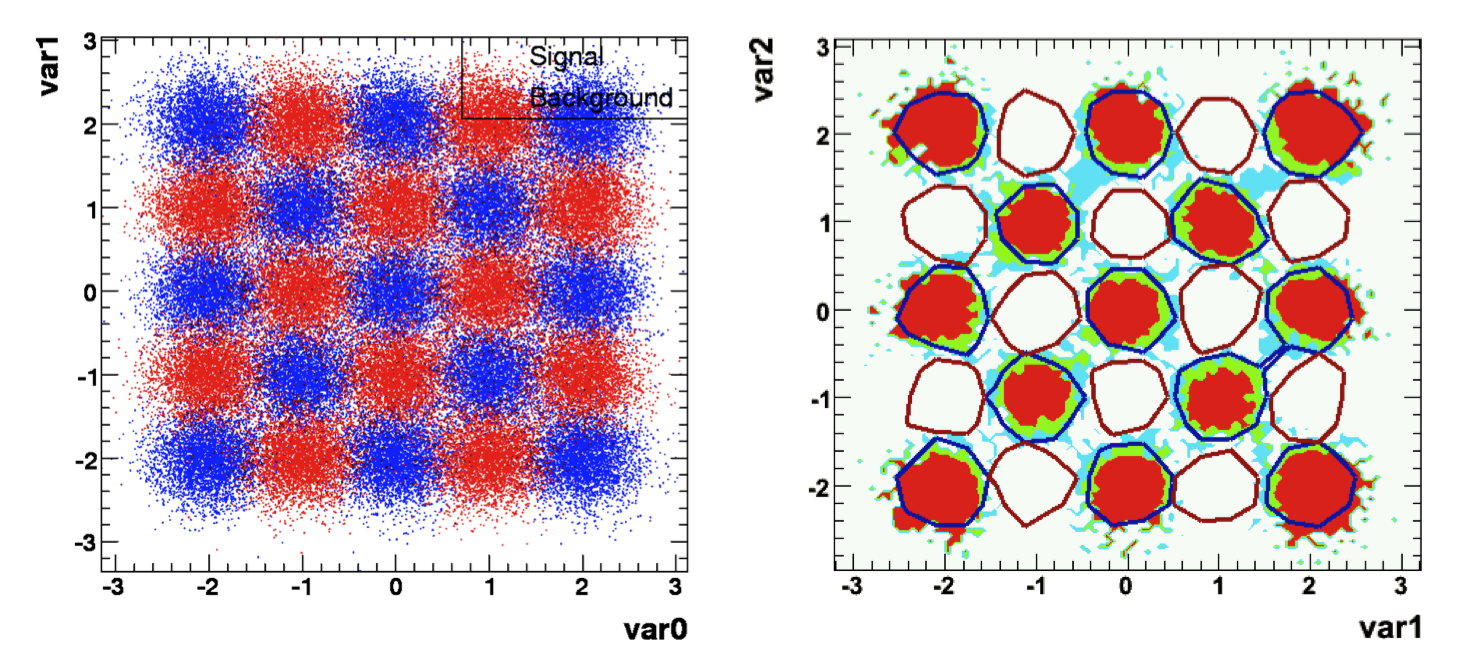
\includegraphics[width=1.00\textwidth]{plots/Schachbrett_both.png}

  \vspace{0.5cm}
  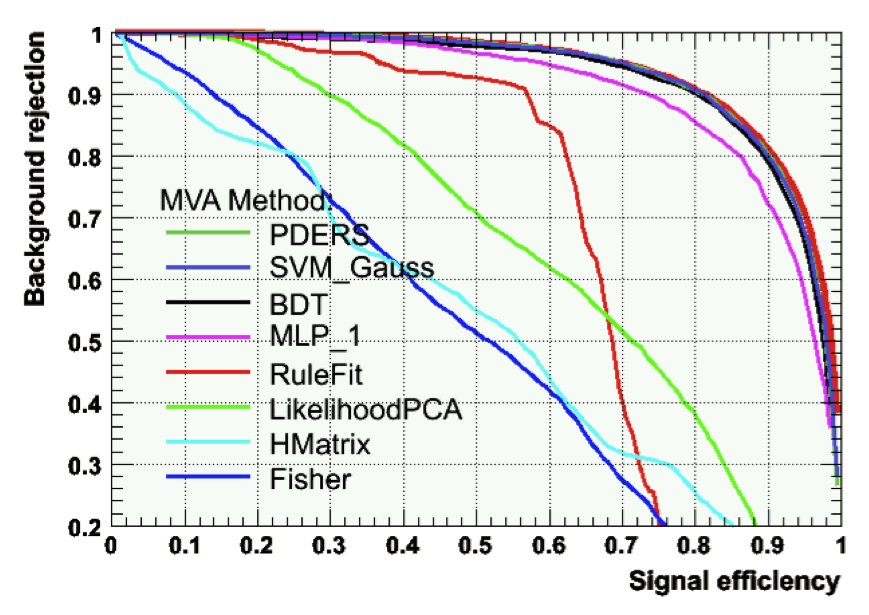
\includegraphics[width=0.65\textwidth]{plots/Schachbrett_ROC.png}
\end{center}
\caption[.]{The top left plot shows the two-dimensional Gaussian-distributed 
  signal (blue) and background (red) distributions for the ``Schachbrett'' toy 
  Monte Carlo sample. In the top right plot is drawn as an example the Support Vector
  Machine's classification response in terms of the weights given to events in
  the two dimensional plane. Dark red signifies large MVA output values,
  \ie\   signal like event regions. The bottom plot gives the ROC curves 
  obtained with several TMVA classifiers for this example after training. 
  The theoretically best ROC curve is known and shown by the thick red outer
  line.  While all the non-linear classification methods (after
  carefully tuning their parameters) are able to approximate the
  theoretical limit, the linear methods strongly underperform. }
\label{fig:conclusions:schachbrett}
\end{figure}

For another academic toy Monte Carlo example however, which exhibits strongly non-linear 
correlations in form of a ``Schachbrett'' (chess board with two-dimensional 
Gaussian-distributed signal and background spots -- see Fig.~\ref{fig:conclusions:schachbrett}), 
the limitations of the linear classifiers, being unable to capture the features of the data,
become manifest. Non-linear classifiers, once appropriately optimised such as choosing 
a sufficiently complex network architecture for the MLP, or the proper kernel functions 
in the SVM, all non-linear methods reproduce or approximate the theoretical limit of 
this classification problem (indicated by the thick red line in the ROCc curve in 
the lower plot of Fig.~\ref{fig:conclusions:schachbrett}).

\section{TMVA implementation status summary for classification and regression}
\label{sec:classifierSummary}

All TMVA methods are fully operational for user analysis, requiring training, testing,
evaluating and reading for the application to unknown data samples. Additional 
features are optional and -- despite our attempts to provide a fully transparent analysis
-- not yet uniformly available. A status summary is given in Table~\ref{tab:methodStatus}
and annotated below.

Although since TMVA 4 the framework supports multi-dimensional MVA outputs it has not yet 
been implemented for classification. For regression, only a few methods are fully multi-target 
capable so far (see Table \ref{tab:methodStatus}). 

Individual event-weight support is now commonly realised, only missing (and not 
foreseen to be provided) for the less recommended neural network CFMlpANN. Support of
negative event weights occurring, \eg, in NLO MC requires more scrutiny as discussed in 
Sec.~\ref{sec:NegativeEventWeights} on page~\pageref{sec:NegativeEventWeights}.

Ranking of the input variables cannot be defined in a straightforward manner for all 
MVA methods. Transparent and objective variable ranking through performance comparison 
of the MVA method under successive elimination of one input variable at a time is under 
consideration (so far only realised for the naive-Bayes likelihood classifier).

Standalone C++ response classes (not required when using the Reader application) 
are generated by the majority of the classifiers, but not yet for regression analysis. 
The missing ones for PDE-RS, PDE-Foam, k-NN, Cuts and CFMlpANN will only be considered on explicit request.

The availability of help messages, which assist the user with the performance tuning 
and which are printed on standard output when using the booking option 'H', is 
complete. 

Finally, custom macros are provided for some MVA methods to analyse specific 
properties, such as the fidelity of likelihood reference distributions or the 
neural network architecture, etc. More macros can be added upon user request.
\begin{sidewaystable}
\begin{center}
{\small
\setlength{\tabcolsep}{0.3pc}
\begin{tabular}{lcccccccccccccc}\hline
&&&&&&&\\[\BD]
                     & Classi- & Regress- & \mc{2}{c}{Multi-class/target} & \mc{2}{c}{Treats event weights:}  & Variable & Standalone & Help & Custom \\
\rs{MVA method}      & fication
                            & ion 
                                   & classification
                                          & regression
                                                 &  positive 
                                                        & negative 
                                                               & ranking 
                                                                      & response class  
                                                                             & messages 
                                                                                    & macros\\[\AD]
\hline
&&&&&&&\\[\BD]
Cut optimisation     & \YES & \NO  & \NO  & \NO  & \YES & \NO  & \NO  & \NO  & \YES & \NO  \\[\AD]
Likelihood           & \YES & \NO  & \NO  & \NO  & \YES & \YES & \YES & \YES & \YES & \YES \\
PDE-RS               & \YES & \YES & \NO  & \NO  & \YES & \YES & \NO  & \NO  & \YES & \NO  \\
PDE-Foam             & \YES & \YES & \YES & \YES & \YES & \YES & \YES & \NO  & \YES & \YES \\
k-NN                 & \YES & \YES & \NO  & \YES & \YES & \YES & \NO  & \NO  & \YES & \NO  \\[\AD]
H-Matrix             & \YES & \NO  & \NO  & \NO  & \YES & \NO  & \YES & \YES & \YES & \NO  \\
Fisher               & \YES & \NO  & \NO  & \NO  & \YES & \NO  & \YES & \YES & \YES & \NO  \\
LD                   & \YES & \YES & \NO  & \NO  & \YES & \NO  & \YES & \YES & \YES & \NO  \\
FDA                  & \YES & \YES & \NO  & \NO  & \YES & \NO  & \NO  & \YES & \YES & \NO  \\[\AD]
MLP                  & \YES & \YES & \NO  & \YES & \YES & \NO  & \YES & \YES & \YES & \YES \\
TMlpANN$^{(\star)}$   & \YES & \NO  & \NO  & \NO  & \YES & \NO  & \NO  & \YES & \YES & \NO  \\
CFMlpANN             & \YES & \NO  & \NO  & \NO  & \NO  & \NO  & \NO  & \NO  & \NO  & \NO  \\[\AD]
SVM                  & \YES & \NO  & \NO  & \NO  & \YES & \YES & \NO  & \YES & \YES & \NO  \\[\AD]
BDT                  & \YES & \YES & \NO  & \NO  & \YES & \YES & \YES & \YES & \YES & \YES \\
RuleFit              & \YES & \NO  & \NO  & \NO  & \YES & \NO  & \YES & \YES & \YES & \YES \\[\AD]
\hline      
&&&&&&&\\[\BD]
\end{tabular}
}
\end{center}
\vspace{-0.4cm}
\footnotesize \hspace{0.8cm}$^{(\star)}$Not a generic TMVA method $-$ interface to ROOT class 
               \code{TMultiLayerPerceptron}.
\caption[.]{\captionfont Status of the methods with respect to various TMVA features. See 
            text for comments. Note that the column ``Standalone response class'' only refers
            to classification. It is yet unavailable for regression. }
\label{tab:methodStatus}
\end{sidewaystable}

\section{Conclusions and Plans}
\label{sec:conclusions}

TMVA is a toolkit that unifies highly customisable multivariate (MVA) classification and 
regression algorithms in a single framework thus ensuring convenient use and an objective 
performance assessment. It is designed for machine learning applications in high-energy 
physics, but not restricted to these. Source code and library of TMVA-v.3.5.0 and higher
versions are part of the standard ROOT distribution kit (v5.14 and higher). The 
newest TMVA development version can be downloaded from Sourceforge.net at 
\urlsm{http://tmva.sourceforge.net}.

This Users Guide introduced the main steps of a TMVA analysis allowing a user to optimise 
and perform her/his own multivariate classification or regression. Let us recall the main 
features of the TMVA design and purpose:
\begin{itemize}

\item TMVA works in transparent factory mode to allow an unbiased 
      performance assessment and comparison: all MVA methods
      see the same training and test data, and are evaluated following 
      the same prescription. 

\item A complete TMVA analysis consists of two steps:
      \begin{enumerate}

      \item {\bf Training:}
            the ensemble of available and optimally customised MVA methods are 
            trained and tested on independent signal and background data samples; the 
            methods are evaluated and the most appropriate (performing and concise) 
            ones are selected.

      \item {\bf Application:}
            selected trained MVA methods are used for the classification of data samples with
            unknown signal and background composition, or for the estimate of unknown 
            target values (regression).  

      \end{enumerate}
      
\item A Factory class object created by the user organises the 
      customisation and interaction with the MVA methods for the training, 
      testing and evaluation phases of the TMVA analysis. The training results 
      together with the configuration of the methods are written to
      result (``weight'') files in XML format.

\item Standardised outputs during the Factory running, and dedicated ROOT 
      macros allow a refined assessment of each method's behaviour and 
      performance for classification and regression.
     
\item Once appropriate methods have been chosen by the user, they can be 
      applied to data samples with unknown classification or target values. Here, 
      the interaction with the methods occurs through a Reader class 
      object created by the user. A method is booked by giving the path to its
      weight file resulting from the training stage. Then, inside
      the user's event loop, the MVA response is returned by the Reader for 
      each of the booked MVA method, as a function of the event values of the 
      discriminating variables used as input for the classifiers. Alternatively,
      for classification, the user may request from the Reader the probability 
      that a given event belongs to the signal hypothesis and/or the event's Rarity.

\item In parallel to the XML files, TMVA generates standalone C++ classes after the 
      training, which can be used for classification problems (feature not available 
      yet for regression). Such classes are available for all classifiers except for 
      cut optimisation, PDE-RS, PDE-Foam, k-NN and the old CFMlpANN.

\end{itemize}
We give below a summary of the TMVA methods, outlining the current state of their
implementation, their advantages and shortcomings.
\begin{itemize}

\item {\em Rectangular Cut Optimisation} \\
      The current implementation is mature. 
      It includes speed-optimised range searches using binary 
      trees, and three optimisation algorithms: Monte Carlo sampling,
      a Genetic Algorithm and Simulated Annealing. In spite of these 
      tools, optimising the cuts for a large number of discriminating variables 
      remains challenging. The user is advised to reduce the available 
      dimensions to the most significant variables (\eg, using a principal
      component analysis) prior to optimising the cuts.

\item {\em Likelihood} \\
      Automatic non-parametric probability density function (PDF) estimation through 
      histogram smoothing and interpolation with various spline functions and 
      quasi-unbinned kernel density estimators is implemented. The PDF description
      can be individually tuned for each input variable. 

\item {\em PDE-RS} \\
      The multidimensional probability density estimator (PDE) approach is in an advanced 
      development stage featuring adaptive range search, several kernel estimation 
      methods, and speed optimised range search using event sorting in binary trees.
      It has also been extended to regression.

\item {\em PDE-Foam} \\
      This new multidimensional PDE algorithm uses self-adapting phase-space 
      binning and is a fast realisation of PDE-RS in fixed volumes, which are
      determined and optimised during the training phase. Much work went 
      into the development of PDE-Foam. It has been thoroughly tested, and 
      can be considered a mature method. PDE-Foam performs classification 
      and regression analyses.

\item {\em k-NN} \\
      The k-Nearest Neighbour classifier is also in a mature state, featuring
      both classification and regression.
      The code has been well tested and shows satisfactory results. 
      With scarce training statistics it may slightly underperform in comparison
      with PDE-RS, whereas it is significantly faster in the application to large
      data samples.

\item {\em Fisher and H-Matrix}\\
      Both are mature algorithms, featuring linear discrimination for classification 
      only. Higher-order correlations are taken care of by FDA (see below).

\item {\em Linear Discriminant (LD)}\\
      LD is equivalent to Fisher but providing both classification and linear 
      regression.

\item {\em Function Discriminant Analysis (FDA)} \\
      FDA is a mature algorithm, which has not been extensively used yet. It 
      extends the linear discriminant to moderately non-linear correlations that
      are fit to the training data.

\item {\em Artificial Neural Networks} \\
      Significant work went into the 
      implementation of fast feed-forward multilayer perceptron algorithms
      into TMVA. Two external ANNs have been integrated as fully independent
      methods, and another one has been newly developed for TMVA, with emphasis 
      on flexibility and speed. The performance of the latter ANN (MLP) has been 
      cross checked against the Stuttgart ANN (using as an example $\tau$ 
      identification in ATLAS), and was found to achieve competitive performance.
      The MLP ANN also performs multi-target regression.

\item {\em Support Vector Machine}\\
      SVM is a relatively new multivariate analysis algorithm with a strong 
      statistical background. It performs well for nonlinear discrimination 
      and is insensitive to overtraining. Optimisation is 
      straightforward due to a low number of adjustable parameters (only two 
      in the case of Gaussian kernel). The response speed is slower than 
      for a not-too-exhaustive neural network, but comparable with other 
      nonlinear methods. SVM is being extended to multivariate regression.

\item {\em Boosted Decision Trees}\\
      The BDT implementation has received constant attention over the years of
      its development. The current version includes additional features like 
      bagging or gradient boosting, and manual or automatic pruning of 
      statistically insignificant nodes. It is a highly performing MVA method
      that also applies to regression problems. 

\item {\em RuleFit} \\
      The current version has the possibility to run either the original 
      program written by J.~Friedman~\cite{RuleFit} or an independent TMVA 
      implementation. The TMVA version has been improved both in speed and 
      performance and achieves almost equivalent results with respect to the 
      original one, requiring however somewhat more tuning.

\end{itemize}

The new framework introduced with TMVA~4 provides the flexibility to combine
MVA methods in a general fashion. Exploiting these capabilities for classification
and regression however requires to create so-called committee methods for each 
combination. So far, we provide a generalised Boost method, allowing to boost
any classifier by simply setting the variable \code{Boost_Num} in the configuration
options to a positive number (plus possible adjustment of other configuration
parameters). The result is a potentially powerful committee method unifying
the excellent properties of boosting with MVA methods that already represent 
highly optimised algorithms. 

Boosting is not the only combination the new framework allows us to establish. 
TMVA now also supports the categorisation of classification according to
the phase space, which allows a better modelling and hence simplifies the 
mapping of the feature space. This particularly improves simple methods, such 
las projective likelihood and linear discriminants. 

\subsubsection*{Acknowledgements}
\addcontentsline{toc}{section}{Acknowledgements}
\label{sec:Acknowledgments}

\begin{details}
The fast growth of TMVA would not have been possible without the 
contribution and feedback from many developers (also co-authors of this Users Guide)
and users to whom we are indebted. 
%
We thank in particular the CERN Summer students Matt Jachowski (Stanford U.) for the 
implementation of TMVA's MLP neural network, and Yair Mahalalel (Tel Aviv U.) for a 
significant improvement of PDE-RS. The Support Vector Machine has been contributed to 
TMVA by Andrzej Zemla and Marcin Wolter (IFJ PAN Krakow), and the k-NN method has 
been written by Rustem Ospanov (Texas U.). 
%
We are grateful to
%
Lucian Ancu,
Doug Applegate, 
Kregg Arms, 
Ren\'e Brun and the ROOT team, 
Andrea Bulgarelli,
Marc Escalier,
Zhiyi Liu, 
Colin Mclean,
Elzbieta Richter-Was, 
Alfio Rizzo,
Lydia Roos,
Vincent Tisserand,
Alexei Volk,
Jiahang Zhong
%
for helpful feedback and bug reports. Thanks also to Lucian Ancu for 
improving the plotting macros.
\end{details}
